%package list
\documentclass{article}
\usepackage[top=3cm, bottom=3cm, outer=3cm, inner=3cm]{geometry}
\usepackage{multicol}
\usepackage{graphicx}
\usepackage{url}
%\usepackage{cite}
\usepackage{hyperref}
\usepackage{array}
%\usepackage{multicol}
\newcolumntype{x}[1]{>{\centering\arraybackslash\hspace{0pt}}p{#1}}
\usepackage{natbib}
\usepackage{pdfpages}
\usepackage{multirow}
\usepackage[normalem]{ulem}
\useunder{\uline}{\ul}{}
\usepackage{svg}
\usepackage{xcolor}
\usepackage{listings}
\lstdefinestyle{ascii-tree}{
    literate={├}{|}1 {─}{--}1 {└}{+}1 
  }
\lstset{basicstyle=\ttfamily,
  showstringspaces=false,
  commentstyle=\color{red},
  keywordstyle=\color{blue}
}
%\usepackage{booktabs}
\usepackage{caption}
\usepackage{subcaption}
\usepackage{float}
\usepackage{array}

\newcolumntype{M}[1]{>{\centering\arraybackslash}m{#1}}
\newcolumntype{N}{@{}m{0pt}@{}}


%%%%%%%%%%%%%%%%%%%%%%%%%%%%%%%%%%%%%%%%%%%%%%%%%%%%%%%%%%%%%%%%%%%%%%%%%%%%
%%%%%%%%%%%%%%%%%%%%%%%%%%%%%%%%%%%%%%%%%%%%%%%%%%%%%%%%%%%%%%%%%%%%%%%%%%%%
\newcommand{\itemEmail}{William Herderson Choquehuanca Berna}
\newcommand{\itemStudent}{Roni Companocca Checco
Franco Jesus Cahua Soto}
\newcommand{\itemCourse}{}
\newcommand{\itemCourseCode}{}
\newcommand{\itemSemester}{II}
\newcommand{\itemUniversity}{Universidad Nacional de San Agustín de Arequipa}
\newcommand{\itemFaculty}{Facultad de Ingeniería de Producción y Servicios}
\newcommand{\itemDepartment}{Departamento Académico de Ingeniería de Sistemas e Informática}
\newcommand{\itemSchool}{Escuela Profesional de Ingeniería de Sistemas}
\newcommand{\itemAcademic}{2023 - B}
\newcommand{\itemInput}{Del 10 de Enero 2024}
\newcommand{\itemOutput}{Al 11 Enero 2024}
\newcommand{\itemPracticeNumber}{01}
\newcommand{\itemTheme}{Composicion-Agregacion}
%%%%%%%%%%%%%%%%%%%%%%%%%%%%%%%%%%%%%%%%%%%%%%%%%%%%%%%%%%%%%%%%%%%%%%%%%%%%
%%%%%%%%%%%%%%%%%%%%%%%%%%%%%%%%%%%%%%%%%%%%%%%%%%%%%%%%%%%%%%%%%%%%%%%%%%%%

\usepackage[english,spanish]{babel}
\usepackage[utf8]{inputenc}
\AtBeginDocument{\selectlanguage{spanish}}
\renewcommand{\figurename}{Figura}
\renewcommand{\refname}{Referencias}
\renewcommand{\tablename}{Tabla} %esto no funciona cuando se usa babel
\AtBeginDocument{%
	\renewcommand\tablename{Tabla}
}

\usepackage{fancyhdr}
\pagestyle{fancy}
\fancyhf{}
\setlength{\headheight}{30pt}
\renewcommand{\headrulewidth}{1pt}
\renewcommand{\footrulewidth}{1pt}
\fancyhead[L]{\raisebox{-0.2\height}{
\includegraphics[width=3cm]{logo_episunsa.png}}}
\fancyhead[C]{\fontsize{7}{7}\selectfont	\itemUniversity \\ \itemFaculty \\ \itemDepartment \\ \itemSchool \\ \textbf{\itemCourse}}
\fancyhead[R]{\raisebox{-0.2\height}{
\includegraphics[width=1.2cm]{abet.png}}}
\fancyfoot[L]{sistema para ingresar datos de alumnos universitarios.}
\fancyfoot[C]{\itemCourse}
\fancyfoot[R]{Página \thepage}

% para el codigo fuente
\usepackage{listings}
\usepackage{color, colortbl}
\definecolor{dkgreen}{rgb}{0,0.6,0}
\definecolor{gray}{rgb}{0.5,0.5,0.5}
\definecolor{mauve}{rgb}{0.58,0,0.82}
\definecolor{codebackground}{rgb}{0.95, 0.95, 0.92}
\definecolor{tablebackground}{rgb}{0.8, 0, 0}

\lstset{frame=tb,
	language=bash,
	aboveskip=3mm,
	belowskip=3mm,
	showstringspaces=false,
	columns=flexible,
	basicstyle={\small\ttfamily},
	numbers=none,
	numberstyle=\tiny\color{gray},
	keywordstyle=\color{blue},
	commentstyle=\color{dkgreen},
	stringstyle=\color{mauve},
	breaklines=true,
	breakatwhitespace=true,
	tabsize=3,
	backgroundcolor= \color{codebackground},
}

\begin{document}
	
	\vspace*{10px}
	
	\begin{center}	
		\fontsize{17}{17} \textbf{ Informe de Practica \itemPracticeNumber}
	\end{center}
	\centerline{\textbf{\Large Tema: \itemTheme}}
	%\vspace*{0.5cm}	

	\begin{flushright}
		\begin{tabular}{|M{2.5cm}|N|}
			\hline 
			\rowcolor{tablebackground}
			\color{white} \textbf{Nota}  \\
			\hline 
			     \\[30pt]
			\hline 			
		\end{tabular}
	\end{flushright}	

	\begin{table}[H]
		\begin{tabular}{|x{4.7cm}|x{4.8cm}|x{4.8cm}|}
			\hline 
			\rowcolor{tablebackground}
			\color{white} \textbf{Integrantes} & \color{white}\textbf{Escuela}  & \color{white}\textbf{Asignatura}   \\
			\hline 
			{\itemStudent \par \itemEmail} & \itemSchool & {\itemCourse \par Semestre: \itemSemester \par Código: \itemCourseCode}     \\
			\hline 			
		\end{tabular}
	\end{table}		
	
	\begin{table}[H]
		\begin{tabular}{|x{4.7cm}|x{4.8cm}|x{4.8cm}|}
			\hline 
			\rowcolor{tablebackground}
			\color{white}\textbf{Practica} & \color{white}\textbf{Tema}  & \color{white}\textbf{Duración}   \\
			\hline 
			\itemPracticeNumber & \itemTheme & 02 horas   \\
			\hline 
		\end{tabular}
	\end{table}
	
	\begin{table}[H]
		\begin{tabular}{|x{4.7cm}|x{4.8cm}|x{4.8cm}|}
			\hline 
			\rowcolor{tablebackground}
			\color{white}\textbf{Semestre académico} & \color{white}\textbf{Fecha de inicio}  & \color{white}\textbf{Fecha de entrega}   \\
			\hline 
			\itemAcademic & \itemInput &  \itemOutput  \\
			\hline 
		\end{tabular}
	\end{table}

    \section{TAREA}
	\begin{itemize}	
    \item SUCURSALES: La biblioteca dispone de varios locales a los que llama sucursales. Se dispone de uno o varios ejemplares de cada libro, que se encuentran distribuidas por las sucursales. Les interesaría saber por cada libro el número de ejemplares asignados a cada sucursal, y el identificador y nombre únicos de la sucursal junto a la dirección de la sucursal. Se deben hacer consultas por autores y almacenar los autores de cada libro. Puede ocurrir que hayan autores diferentes que se llamen igual. Se debe distinguir a dos autores con el mismo nombre por el libro del que son autores. No puede haber dos autores con el mismo nombre que hayan escrito el mismo libro (distinguiendo a los libros por su identificador único).


    \end{itemize}

    \section{EQUIPOS, MATERIALES Y TEMAS UTILIZADOS}
	\begin{itemize}
		\item Sistema Operativo Windows
		\item OpenJDK 64-Bits 17.0.7.
		\item Git 2.39.2.	
  	\item Cuenta en GitHub con el correo institucional.
	\end{itemize}

    \section{URL DE REPOSITORIO GITHUB}
	\begin{itemize}
		\item URL para el Repositorio GitHub.
		\item \url{https://github.com/RONI-COMPANOCCA-CHECCO}
		\item URL para la practica 01 en el Repositorio GitHub.	
        \item \url{https://github.com/RONI-COMPANOCCA-CHECCO/PRACTICA01-FASE03}
	\end{itemize}
    
    \section{EJERCICIO}
	\begin{itemize}
 \item son los codigos que creamos y a los que modificamos para que nuestro programa compile adecuadamente.
        \subsection{Clase Branch.java la clase sucursal}

        \begin{lstlisting}[language=java]
import java.util.HashMap;

public class Branch {
    private String id;
    private String name;
    private String address;
    private HashMap<Book, Integer> bookCopies;

    public Branch(String id, String name, String address) {
        this.id = id;
        this.name = name;
        this.address = address;
        this.bookCopies = new HashMap<>();
    }

    public String getId() {
        return id;
    }

    public String getName() {
        return name;
    }

    public String getAddress() {
        return address;
    }

    public void addBookCopy(Book book, int copies) {
        bookCopies.put(book, copies);
    }

    public int getBookCopies(Book book) {
        return bookCopies.getOrDefault(book, 0);
    }
    public void printBranchInfo() {
        System.out.println("Sucursal: " + getName());
        System.out.println("ID: " + getId());
        System.out.println("Direcci�n: " + getAddress());
        System.out.println("Libros en la sucursal:");

        for (Book book : bookCopies.keySet()) {
            int copies = bookCopies.get(book);
            System.out.println(" - Libro: " + book.getTitle() + ", Ejemplares: " + copies);
        }
    }
}

        \end{lstlisting}

        \subsection{Clase Author.java}

        \begin{lstlisting}[language=java]
public class Author {
    private String name;
    private String code;

    public Author(String name) {
        this.name = name;
        this.code = code;
    }

    public String getName() {
        return name;
    }

    public String getCode() {
        return code;
    }
}
        \end{lstlisting}

        \subsection{Clase Editorial.java}

        \begin{lstlisting}[language=java]
import java.util.ArrayList;
import java.util.HashMap;
import java.util.List;
import java.util.Map;

public class Editorial {
	private String name;
    private String webPage;
    private boolean status;
    private ArrayList<Article> articles;
    private ArrayList<Branch> branches;
    private ArrayList<Author> authors;
    private Map<Author, List<Book>> authorBooks;

	public Editorial(String name) {
        this.name = name;
        this.articles = new ArrayList<>();
        this.branches = new ArrayList<>();
        this.authors = new ArrayList<>();
        this.authorBooks = new HashMap<>();
    }

	public String getName() {
		return name;
	}
	public void setName(String name) {
		this.name = name;
	}
	public String getWebPage() {
		return webPage;
	}
	public void setWebPage(String webPage) {
		this.webPage = webPage;
	}
	public boolean isStatus() {
		return status;
	}
	public void setStatus(boolean status) {
		this.status = status;
	}
	
	public boolean addArticle(Article article) {
        if (articles.contains(article)) {
            return false;
        } else {
            this.articles.add(article);

            if (article instanceof Book) {
                Author author = ((Book) article).getAuthor();
                if (!authors.contains(author)) {
                    authors.add(author);
                }

                // Almacenar el libro bajo el autor
                authorBooks.computeIfAbsent(author, k -> new ArrayList<>()).add((Book) article);
            }

            return true;
        }
    }

	public boolean addBranch(Branch branch) {
        if (branches.contains(branch)) {
            return false;
        } else {
            branches.add(branch);
            return true;
        }
    }	
	
	public boolean searchBooks(String code) {
		for(int i=0;i<articles.size();i++) {
			if(articles.get(i).getCode().equals(code)) {
				return true;
			}
		}
		return false;
	}
	public ArrayList<Article> getArticles() {
		return articles;
	}
	
	public void printArticles() {
		for (Article article : articles) {
            System.out.println("Editorial: " + this.getName());
            System.out.println("------------------------");
            System.out.println("Código: " + article.getCode());
            System.out.println("Título: " + article.getTitle());
            System.out.println("Páginas: " + article.getPages());
            System.out.println("Autor: " + ((Book) article).getAuthor().getName());
            System.out.println("\n");

            /*if (article instanceof Book) {
                System.out.println("ISBN: " + ((Book) article).getISBN());
                System.out.println("Autor: " + ((Book) article).getAuthor().getName());
            } else if (article instanceof Thesis) {
              
            } else if (article instanceof Journal) {
     
            }*/
   
        }
		
	}
    public void printAuthorBooks() {
        System.out.println("\n----Libros por Autor:----");

        for (Author author : authorBooks.keySet()) {
            System.out.println("Autor: " + author.getName());
            List<Book> books = authorBooks.get(author);
            
            for (Book book : books) {
                System.out.println(" - Libro: " + book.getTitle());
            }
        }
    }
		
}
        \end{lstlisting}
        
        \subsection{Clase Main.java}

        \begin{lstlisting}[language=java]
public class Main {
    public static void main(String[] args) {
        Editorial e1 = new Editorial("UNIVERSIDAD");
        Author author1 = new Author("Robert C. Martin");
        Author author2 = new Author("Marijn Haverbeke");
        Author author3 = new Author("Kyle Simpson");
        Book b1 = new Book("F23-678","Clean Code", author1, 358);
        Book b2 = new Book("F78-098","Eloquent JavaScript", author2, 250);
        b2.setISBN("978-612-00-0855-3");
        Book b3 = new Book("F67-908","You dont know JavaScript", author3, 410);
        Book b4 = new Book("K58-098","Clean Agile: Back to Basics", author1, 350);
        Book b5 = new Book("K68-098","Agile Software Development", author1, 950);
        Thesis t1 = new Thesis("THESIS-ISIS-01", "Modelo de Analisis del sentimiento en la Red Social Facebook usando Redes Neuronales", 118);
        Journal j1 = new Journal("JOURNAL-ISIS-01", "Revista de la Escuela Profesional de Ingenieria de Sistemas", 80);

        Branch branch1 = new Branch("BRANCH-001", "Sucursal A", "Direccion A");
        Branch branch2 = new Branch("BRANCH-002", "Sucursal B", "Direccion B");
        Branch branch3 = new Branch("BRANCH-003", "Sucursal C", "Direccion C");
        Branch branch4 = new Branch("BRANCH-004", "Sucursal D", "Direccion D");

        System.out.println((e1.addArticle(b1)) ? "Exito" : "Fracaso");
        System.out.println((e1.addArticle(b2)) ? "Exito" : "Fracaso");
        System.out.println((e1.addArticle(b3)) ? "Exito" : "Fracaso");
        System.out.println((e1.addArticle(b4)) ? "Exito" : "Fracaso");
        System.out.println((e1.addArticle(b5)) ? "Exito" : "Fracaso");
        e1.printArticles();
        
        branch1.addBookCopy(b1, 5);
        branch1.addBookCopy(b2, 3);
        branch1.addBookCopy(b3, 7);
        branch1.addBookCopy(b4, 12);
        branch2.addBookCopy(b1, 7);
        branch2.addBookCopy(b2, 2);
        branch2.addBookCopy(b3, 8);
        branch2.addBookCopy(b5, 18);
        branch3.addBookCopy(b1, 7);
        branch3.addBookCopy(b2, 2);
        branch3.addBookCopy(b3, 8);
        branch3.addBookCopy(b4, 17);
        branch4.addBookCopy(b1, 7);
        branch4.addBookCopy(b2, 2);
        branch4.addBookCopy(b3, 8);
        branch4.addBookCopy(b4, 13);
        branch4.addBookCopy(b5, 21);
        
        System.out.println("---INFORMACION DE LAS SUCURSALES---");
        System.out.println("--------------------");
        System.out.println("--------------------");
        branch1.printBranchInfo();
        System.out.println("\n");
        branch2.printBranchInfo();
        System.out.println("\n");
        branch3.printBranchInfo();
        System.out.println("\n");
        branch4.printBranchInfo();
        
        e1.printAuthorBooks();
    }
}

        \end{lstlisting}

        \subsection{EJECUCION}
              
        \begin{lstlisting}[language=java]
Editorial: UNIVERSIDAD
------------------------
Código: F23-678
Título: Clean Code
Páginas: 358
Autor: Robert C. Martin


Editorial: UNIVERSIDAD
------------------------
Código: F78-098
Título: Eloquent JavaScript
Páginas: 250
Autor: Marijn Haverbeke


Editorial: UNIVERSIDAD
------------------------
Código: F67-908
Título: You dont know JavaScript
Páginas: 410
Autor: Kyle Simpson


Editorial: UNIVERSIDAD
------------------------
Código: K58-098
Título: Clean Agile: Back to Basics
Páginas: 350
Autor: Robert C. Martin


Editorial: UNIVERSIDAD
------------------------
Código: K68-098
Título: Agile Software Development
Páginas: 950
Autor: Robert C. Martin


---INFORMACION DE LAS SUCURSALES---
--------------------
--------------------
Sucursal: Sucursal A
ID: BRANCH-001
Direcci?n: Direccion A
Libros en la sucursal:
 - Libro: Clean Code, Ejemplares: 5
 - Libro: Eloquent JavaScript, Ejemplares: 3
 - Libro: You dont know JavaScript, Ejemplares: 7
 - Libro: Clean Agile: Back to Basics, Ejemplares: 12


Sucursal: Sucursal B
ID: BRANCH-002
Direcci?n: Direccion B
Libros en la sucursal:
 - Libro: Clean Code, Ejemplares: 7
 - Libro: Eloquent JavaScript, Ejemplares: 2
 - Libro: Agile Software Development, Ejemplares: 18
 - Libro: You dont know JavaScript, Ejemplares: 8


Sucursal: Sucursal C
ID: BRANCH-003
Direcci?n: Direccion C
Libros en la sucursal:
 - Libro: Clean Code, Ejemplares: 7
 - Libro: Eloquent JavaScript, Ejemplares: 2
 - Libro: You dont know JavaScript, Ejemplares: 8
 - Libro: Clean Agile: Back to Basics, Ejemplares: 17


Sucursal: Sucursal D
ID: BRANCH-004
Direcci?n: Direccion D
Libros en la sucursal:
 - Libro: Clean Code, Ejemplares: 7
 - Libro: Eloquent JavaScript, Ejemplares: 2
 - Libro: Agile Software Development, Ejemplares: 21
 - Libro: You dont know JavaScript, Ejemplares: 8
 - Libro: Clean Agile: Back to Basics, Ejemplares: 13

----Libros por Autor:----
Autor: Robert C. Martin
 - Libro: Clean Code
 - Libro: Clean Agile: Back to Basics
 - Libro: Agile Software Development
Autor: Marijn Haverbeke
 - Libro: Eloquent JavaScript
Autor: Kyle Simpson
 - Libro: You dont know JavaScript
        \end{lstlisting}
        \item Diagrama UML
 
             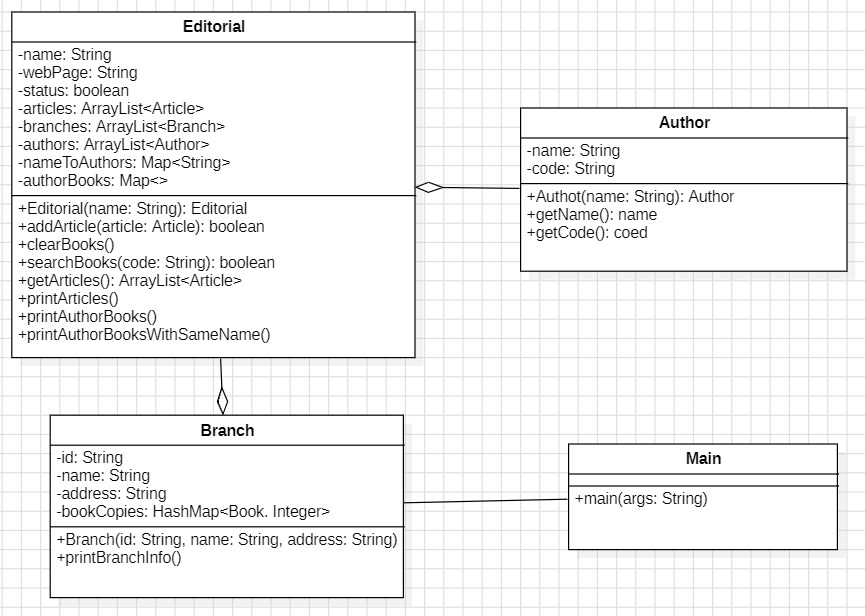
\includegraphics[height=12cm]{uml.jpeg}
	\end{itemize}
	
	\section{REFERENCIAS}
	\begin{itemize}
		\item M. Aedo, “Fundamentos de Programación 2 - Tópicos de Programación Orientada a Objetos”, Primera Edición, 2021, Editorial UNSA.
		\item \url{https://github.com/rescobedoq/programacion.git}
		\item J. Dean, "Introduction to programming with Java: A Problem Solving Approach”, Third Edition, 2021, McGraw-Hill.
        \item C. T. Wu, "An Introduction to Object-Oriented Programming with Java", Fifth Edition, 2010, McGraw-Hill.
        \item P. Deitel, "Java How to Program", Eleventh Edition, 2017, Prentice Hall.
	\end{itemize}
	
%\clearpage
%\bibliographystyle{apalike}
%\bibliographystyle{IEEEtranN}
%\bibliography{bibliography}
			
\end{document}